\chapter{Creación de objetos}


\lettrine[ante=\raisebox{-1.5ex}{\Large ---},lines=2]{M}{irá} ---empezó
Antonia---; para crear, no sé, un cubo, escribís esto:

% \begin{center}
%   \begin{minipage}[]{.5\textwidth}
%     \begin{lstlisting}
% cube([10,20,30]);    
%     \end{lstlisting}
%   \end{minipage}\hfill
%    \begin{minipage}[]{.5\textwidth}
%      \centering
%      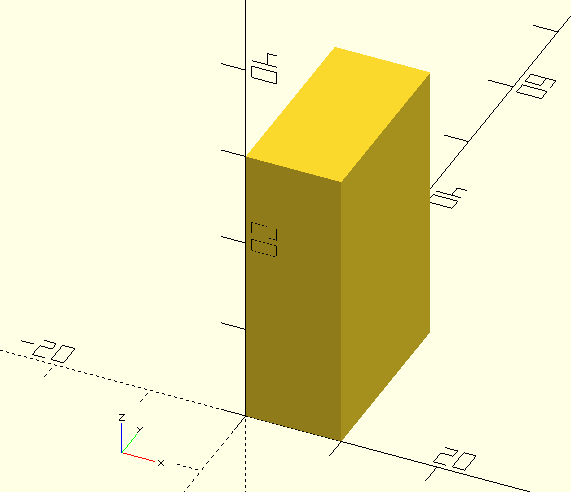
\includegraphics[width=6cm]{cubo}
%    \end{minipage}
%  \end{center}


\begin{lstlisting}[numbers=none]
cube([10,20,30]);    
\end{lstlisting}


\guillemotright Acto seguido, pulsás la tecla \keystroke{F5} para
visualizar el resultado de tan expresiva sentencia ---añadió con un
cierto aire pedagógico.


\begin{figure}[ht]
  \centering
  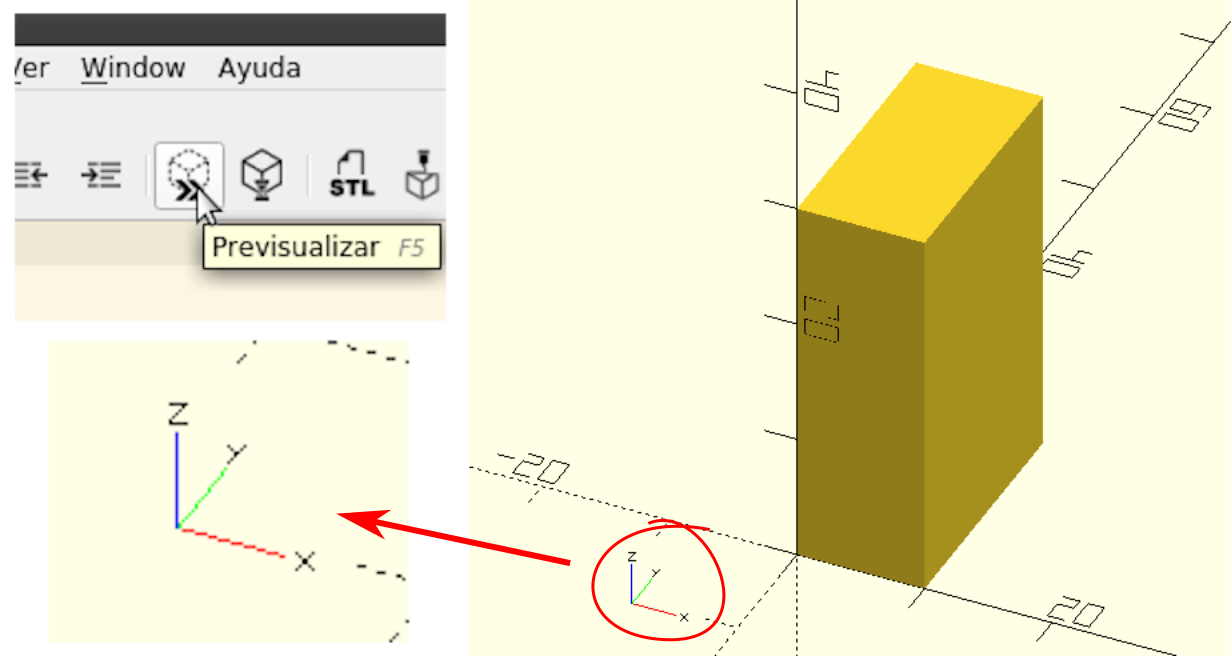
\includegraphics[width=.85\textwidth,valign=c]{imagenes/cubo-f5-flecha}
  \caption{Antonia crea un \lstinline!cube!.}
  \label{fig:cubo}
\end{figure}
 

Cecilia pensó que el objeto recién creado por Antonia no era
precisamente un cubo, pero pudo captar la idea: los valores entre
corchetes indicaban el tamaño de un paralelepípedo recto de base
rectangular en cada uno de los tres ejes cartesianos. En otras
palabras, el objeto medía 10 en \coord{X}, 20 en \coord{Y} y 30 en
\coord{Z}. La identidad de las coordenadas pudo deducirla gracias a
los pequeños ejes cartesianos que se veían abajo a la izquierda en la
figura \ref{fig:cubo}. Por lo demás, decidió ser indulgente con el
nombre del objeto: supuso que a ningún programador le gustaría
escribir \emph{paralelepípedo recto de base rectangular} (aun en
inglés) un número de veces mayor que dos.\footnote{Cecilia parece
  ignorar que en español existe una palabra suficientemente breve que
  designa dicho objeto geométrico: \emph{ortoedro}. (Nota del Editor)}

Antonia continuó:

---Para un cilindro escribís:

\begin{figure}[ht]
  \begin{minipage}[]{.4\textwidth}
    \begin{lstlisting}[numbers=none]
cylinder(h=30,r=10);
    \end{lstlisting}
  \end{minipage}\hfill
   \begin{minipage}[]{.6\textwidth}
     \centering
     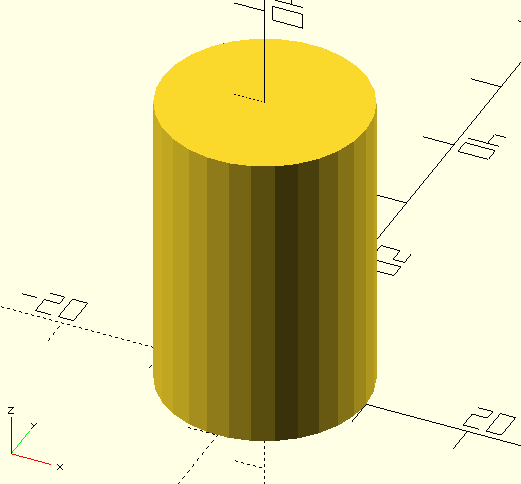
\includegraphics[width=.9\textwidth]{imagenes/cilindro}
   \end{minipage}
  \caption{Antonia crea un \lstinline!cylinder!.}
  \label{fig:cilindro}
\end{figure}


 A Cecilia no le costó mucho desentrañar la lógica de esa línea: un
 cilindro parecía definirse por su altura (\lstinline!h=30!) y su
 radio (\lstinline!r=10!).

 ---Antonia ---preguntó Cecilia---, ¿en qué unidades mide las
 distancias \texttt{OpenSCAD}?

 ---Milímetros ---contestó Antonia.

 ---Lógico ---concedió Cecilia---. Otra cosa: ¿Por qué el supuesto
 cilindro no tiene un contorno debidamente circular, sino facetado?

 ---Es una buena pregunta ---comenzó Antonia, y Cecilia supo entonces
 que iba a tener que fumarse un poco de humo: Antonia sólo consideraba
 buenas aquellas preguntas para las cuales no contaba con una
 respuesta satisfactoria---. El formato de los objetos
 tridimensionales que \texttt{OpenSCAD} produce en última instancia
 ---agregó---, a fin de ser luego impresos en 3D, sólo permite
 acotarlos con superficies planas: triángulos o rectángulos. De esa
 manera, una superficie curva debe ser reducida a un cierto número de
 caras planas.
 
 Cecilia intentó negociar:

 ---Entiendo que pueda ser un tanto ingenuo pretender objetos
 euclideamente cilíndricos, pero ¿no se podría suavizar un poco la
 superficie de ese tubo, al menos a la vista y luego al tacto?

 ---Por supuesto ---Antonia sonrió---; la variable de sistema
 \lstinline!$fn! define la cantidad de caras que una superficie curva
 debe tener; mirá ---agregó, escribiendo rápidamente el ejemplo de la
 figura \ref{fig:cilindro-5000}. %$

 
 \begin{figure}[ht]
  \begin{minipage}[]{.4\textwidth}
    \begin{lstlisting}
$fn=5000;

cylinder(h=30,r=10);
    \end{lstlisting}%$
  \end{minipage}%\hfill
   \begin{minipage}[]{.6\textwidth}
     \centering
     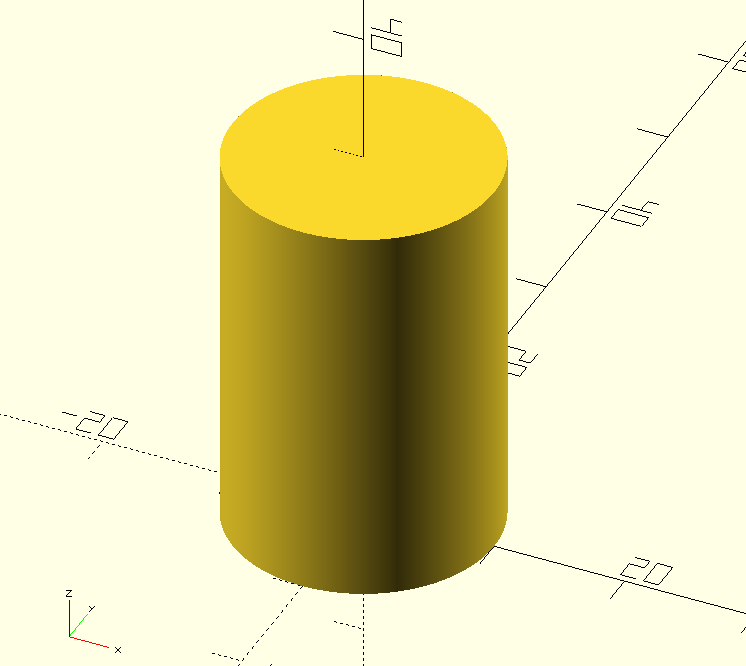
\includegraphics[width=.9\textwidth]{imagenes/cilindro-5000}
   \end{minipage}
   \caption{Antonia crea un \lstinline!cylinder! con un tanto
     exagerado pero indiscutiblemente eficaz
     \lstinline!$fn=5000!.}%$
  \label{fig:cilindro-5000}
\end{figure}

 
\guillemotright Creo que se me fue la mano con 5000 ---confesó Antonia
con una ligera risita---, pero la idea es ésa: con
\lstinline!$fn=5000! le decís a \texttt{OpenSCAD} que los objetos
deben dividir sus partes curvas en 5000 caras.\footnote{Los autores de
  \openscad{} sugieren no emplear valores mayores a 100 para
  \texttt{\$fn}. (Nota del Editor)} En fin, ya debés sospechar cómo se
hace una esfera: %$


\begin{figure}[ht]
  \begin{minipage}[]{.4\textwidth}
    \begin{lstlisting}
$fn=200;
      
sphere(r=10);
    \end{lstlisting}%$
  \end{minipage}\hfill
  \begin{minipage}[]{.6\textwidth}
    \centering
    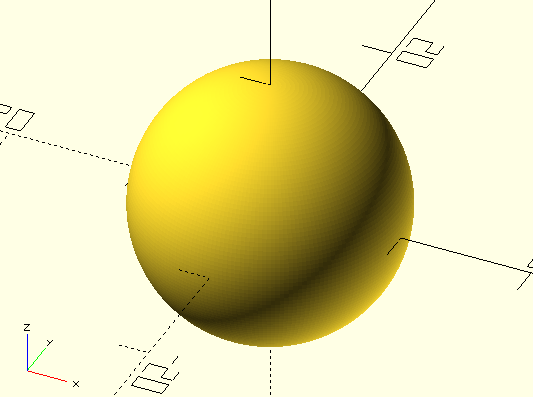
\includegraphics[width=.9\textwidth]{imagenes/esfera}
  \end{minipage}
   \caption{Antonia crea una \lstinline!sphere!.}
  \label{fig:sphere}
\end{figure}


\guillemotright Creo que es un buen momento para pasar algunas ideas
básicas en limpio ---Antonia retomó su tono di\-dác\-ti\-co---. Cada
una de las líneas que escribí hasta ahora puede contemplarse como una
instrucción o sentencia; una suerte de `orden' o `indicación' a
\texttt{OpenSCAD} con un sentido propio. Algunas sirven para crear un
objeto (como \lstinline!cube([10,20,30])!), mientras que otras
advierten acerca de cómo deben concretarse dichos objetos (como
\lstinline!$fn=200!). %$


\guillemotright Las sentencias finalizan con un punto y coma
(\texttt{;}). Las líneas en blanco no tienen otro efecto que organizar
mejor, a la vista, el texto: podés usarlas a discreción.



\guillemotright ¡Ah! ¡Casi me olvidaba! ---soltó con vivacidad
Antonia, y Cecilia no pudo distinguir si estaba o no sobreactuando el
tono de alarma---. Nunca te olvides de grabar tu trabajo: la
combinación \keystroke{Ctrl}+\keystroke{S} debe ser una de tus mejores
aliadas.


\begin{figure}[ht]
  \centering 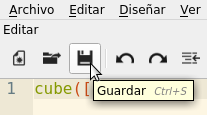
\includegraphics[width=.45\textwidth]{imagenes/guardar}
  \caption{Icono para guardar el texto.}
  \label{fig:guardar}%\iftoggle{libro}{}{\vspace{128in}}
\end{figure}

Cecilia no pudo evitar un leve bostezo.




%%% Local Variables:
%%% mode: latex
%%% TeX-master: "../libro"
%%% End:
